\documentclass[twoside]{report}
\usepackage[italian]{babel}
\usepackage[utf8]{inputenc}
\usepackage{amsmath}
\usepackage{amsthm}
\usepackage{amsfonts}
\usepackage{amssymb}
\usepackage{cancel}
\usepackage[margin=1in]{geometry}
\usepackage{hyperref}
\usepackage{bookmark}
\usepackage{setspace}
\usepackage{titlesec}
\usepackage{fancyhdr}
\usepackage{adjustbox}
\usepackage{float}
\usepackage{graphicx}
\usepackage{float}


\setlength{\parskip}{0pt}
\titlespacing*{\subparagraph}{1em}{0em}{0em} 

\makeatletter
\renewenvironment{abstract}{%
    \if@twocolumn
        \section*{\abstractname}%
    \else
        \begin{center}%
            {\bfseries \abstractname\vspace{-.5em}\vspace{\z@}}%
        \end{center}%
        \small
        \begin{quotation}
    \fi}
    {\if@twocolumn\else\end{quotation}\fi}
\makeatother

\hypersetup{
    pdfauthor={Luca Facchini},
    pdftitle={Appunti di Reti},
    pdfsubject={Appunti del corso di Reti, tenuto dal prof. Casari Paolo presso l'Università degli Studi di Trento. Corso seguito nell'anno accademico 2024/2025.},
    pdfkeywords={Reti, Università degli Studi di Trento, Casari Paolo},
    pdfproducer={LaTeX},
    pdfcreator={pdflatex},
}

\fancypagestyle{chapterInit}{%
    \fancyhf{}
    \renewcommand{\headrulewidth}{0pt}
    \renewcommand{\footrulewidth}{0.4pt}
    \fancyfoot{}
    \fancyfoot[LE,RO]{\thepage}
    \fancyfoot[LO,RE]{"Appunti di Reti" di Luca Facchini}
}

\graphicspath{{./images/}}


\title{Appunti di Reti}
\author{Luca Facchini (mat. 245965)}
\date{A.A. 2024/2025}

\begin{document}
    \begin{titlepage}
        \centering  % Center everything on the title page
        {\Huge\textbf{Appunti di Reti}} \\[1cm] % Title
        \vspace{0.5cm}
        
        {\Large Luca Facchini} \\ % Author name
        \vspace{0.3cm}
        {\large Matricola: 245965} \\[2cm] % Additional author info
        
        {\large Corso tenuto dal prof. Casari Paolo} \\[0.3cm] % Course information
        {\large Università degli Studi di Trento} \\[1.5cm]
        
        {\large A.A. 2024/2025} \\[3cm] % Academic year
        
        % Abstract section with spacing control
        \vfill
        \begin{abstract}
            Appunti del corso di Reti, tenuto dal prof. Casari Paolo presso l'Università degli Studi di Trento. Corso seguito nell'anno accademico 2024/2025.
        \end{abstract}
        
        \vfill  % Pushes the content to the center vertically
    \end{titlepage}
    \tableofcontents

    \pagestyle{fancy}
    \fancyhead{}
    \fancyhead[RO,LE]{\leftmark}
    \fancyhead[RE,LO]{\rightmark}
    \fancyfoot{}
    \renewcommand{\footrulewidth}{0.4pt}
    \fancyfoot[LE,RO]{\thepage}
    \fancyfoot[LO,RE]{"Appunti di Reti" di Luca Facchini}
    
    \chapter{Nozioni di base}
Nel seguente capitolo definiamo alcune nozioni di base che verranno utilizzate all'interno del corso.

\paragraph{Sistema di riferimento} Un sistema di riferimento è un insieme di regole che permettono di determinare la posizione di un punto nello spazio. Un sistema di riferimento è composto da un'origine, da un insieme di assi e da un'unità di misura. Definiamo un sistema di riferimento in quattro assi: $x$, $y$, $z$ e $t$ dove $t$ rappresenta il tempo.
\begin{definition}[Spazio-Tempo Euclideo]
    Lo spazio-tempo euclideo ($S$) è un sistema di riferimento in quattro assi, $x$, $y$, $z$ e $t$, dove $t$ rappresenta il tempo. Lo spazio-tempo euclideo è definito come:
    $$
        S(O_z, x, y, z; O_t, t)
    $$
    dove $O_z$ è l'origine degli assi spaziali e $O_t$ è l'origine dell'asse temporale.
\end{definition}

\section{Moti in una dimensione e grafico orario}
    Per descrivere i moti in una dimensione possiamo utilizzare un grafico non affine, quindi non lineare, che rappresenta la posizione di un punto in funzione del tempo. Questo grafico è detto \textit{grafico orario}.
    \begin{definition}[Grafico Orario]
        Il grafico orario è un grafico cartesiano che esprime la posizione di un punto che si muove in una dimensione in funzione del tempo.
    \end{definition}
    \begin{tikzpicture}
        \begin{axis}
            [axis lines = left, xlabel = $t$, ylabel = $x$, xmin = 0, xmax = 11, ymin = 0, ymax = 11, xtick = {0, 2, 10}, ytick = {0, 2, 10}, xticklabels = {$0$, $t_i$, $t_f$}, yticklabels = {$0$, $x_i\ P_i$, $x_f\ P_f$}, legend pos = north west]
            \addplot[mark = *, color = red] coordinates {(2, 2)} node[above] {$E_i$};
            \addplot[mark = *, color = blue] coordinates {(10, 10)} node[above] {$E_f$};
        \end{axis}
    \end{tikzpicture}
    Vediamo come al momento $t_i$ il punto sia in posizione $P_i$ e di verifica come l'evento $E_i$ sia in posizione $x_i$. Al momento $t_f$ il punto è in posizione $P_f$ e l'evento $E_f$ è in posizione $x_f$. Ora possiamo definite lo spostamento:
    \begin{definition}[Spostamento]
        Lo spostamento è la variazione di posizione di un punto in un intervallo di tempo. Lo spostamento è definito come:
        $$
            \begin{aligned}
                S_{i \to f} &= x_f - x_i\\
                \Delta x_{i \to f} &= x_f - x_i
            \end{aligned}
        $$
    \end{definition}
    Da notare come lo spostamento non descrive ne' la traiettoria ne' la distanza percorsa dal punto ma solo la variazione di posizione, infatti il punto potrebbe aver compiuto un percorso "non diretto". Inoltre nello spostamento ha un verso definito e come conseguenza scrivere $S_{i \to f} \neq S_{f \to i}$.
    \begin{definition}[Distanza Percorsa]
        La distanza percorsa è la lunghezza della traiettoria percorsa da un punto in un intervallo di tempo. La distanza percorsa è definita come:
        $$
            d(P_i, P_f) = \left| x_f - x_i \right|
        $$
    \end{definition}
    Notiamo come la distanza percorsa sia sempre positiva in quanto è la lunghezza della traiettoria percorsa dal punto. Inoltre la distanza percorsa non ha un verso definito, infatti $d(P_i, P_f) = d(P_f, P_i)$.\newline
    Ora per descrivere il moto di un punto possiamo definire la velocità media:
    \begin{definition}[Velocità media]
        La velocità media è la variazione di posizione di un punto in funzione del tempo. La velocità media è definita come:
        $$
            \begin{aligned}
                v_m &= \frac{\Delta x}{\Delta t} = \frac{\Delta x_{i \to f}}{\Delta t_{i \to f}}\\
            \end{aligned}
        $$
    \end{definition}
    Da notare come la velocità media non tiene conto del moto del punto in un intervallo di tempo, ma solo della variazione di posizione. Inoltre la velocità media ha un verso definito in quanto trattiamo lo spostamento (il quale ha un verso definito).\newline
    Per descrivere il moto di un punto in un instante $t$ di tempo possiamo definire la velocità istantanea:
    \begin{definition}[Velocità istantanea]
        La velocità istantanea è la variazione di posizione di un punto in un istante di tempo. La velocità istantanea è definita come:
        $$
            v_i(t)=\lim\limits_{\Delta t \to 0} \frac{\Delta x}{\Delta t} = \frac{dx}{dt}
        $$
    \end{definition}
    Dal punto di vista matematico la velocità istantanea è la derivata della posizione rispetto al tempo. Dunque i punti dove si passa da un movimento ``in avanti'' ad un movimento ``all'indietro'' sono i punti in cui la velocità istantanea è nulla ovvero i punti di massimo e minimo della funzione posizione, inoltre il punto in cui la velocità istantanea è nulla è detto punto di inversione. Inoltre la velocità istantanea è una funzione continua in quanto la derivata di una funzione continua è anch'essa continua.\newline
    È vero che in un determinato periodo di tempo io possa aumentare o diminuire la velocità, per questo motivo definiamo la funzione di accelerazione:
    \begin{definition}[Accelerazione]
        L'accelerazione è la variazione di velocità di un punto in funzione del tempo. L'accelerazione è definita come:
        $$
            \begin{aligned}
                a &= \frac{\Delta v}{\Delta t} = \frac{\Delta v_{i \to f}}{\Delta t_{i \to f}}\\
            \end{aligned}
        $$
    \end{definition}
    Da notare come l'accelerazione non tiene conto del moto del punto in un intervallo di tempo, ma solo della variazione di velocità. Inoltre l'accelerazione ha un verso definito in quanto trattiamo la variazione di velocità (la quale ha un verso definito).
    \paragraph{Relazione tra posizione, velocità e accelerazione}
        Come già detto la velocità è la derivata della posizione rispetto al tempo e l'accelerazione è la derivata della velocità rispetto al tempo, è vero inoltre che la posizione è l'integrale della velocità rispetto al tempo e questa è l'integrale dell'accelerazione rispetto al tempo. Dunque possiamo scrivere:
        \begin{align}
            x(t) &\text{ posizione} \\
            v(t) = \frac{dx}{dt} &\text{ velocità} \\
            a(t) = \frac{dv}{dt} = \frac{d^2x}{dt^2} &\text{ accelerazione}
        \end{align} 
        Al contrario possiamo scrivere:
        \begin{align}
            v(t) &= v_0 + \int_{t_0}^{t} a(T) dT\\
            x(t) &= x_0 + \int_{t_0}^{t} v(T) dT = x_0 + \int_{t_0}^{t} dT \left[v_0+\int_{t_0}^{T} a(\tau) d\tau\right]
        \end{align}
        Ora le dimensioni fisiche (e non le unità di misura) di queste grandezze sono:
        $$
            \begin{aligned}
                \left[x\right] &= \left[L\right]\\
                [v] &= \left[\frac{L}{T}\right]\\
                [a] &= \left[\frac{L}{T^2}\right]
            \end{aligned}
        $$
        ed le rispettive unità di misura sono:
        $$
            \begin{aligned}
                \left[x\right] &= \left[m\right]\\
                [v] &= \left[\frac{m}{s}\right]\\
                [a] &= \left[\frac{m}{s^2}\right]
            \end{aligned}
        $$
    \chapter{Il Livello Applicazione}
\thispagestyle{chapterInit}
\section{principi delle applicazioni di rete}
    \subsection{Architetture di rete}
        Esistono varie architetture per le applicazioni di rete, tra le quali:
        \begin{itemize}
            \item Client-Server
            \item Peer-to-Peer
            \item Architetture ibride
            \item Cloud Computing 
        \end{itemize}
        \subsubsection{Client - Server}
        \label{subsubsec:clientServer}
            In questa architettura esistono due ruoli principali:
            \paragraph{Server} Il server è un host \textbf{sempre attivo} con un \textbf{indirizzo permanente} e molto spesso difficile da scalare
            \paragraph{Client} Il client \textbf{comunica col server}, inoltre a differenza del server può \textbf{disconnettersi temporaneamente} e inoltre può avere un \textbf{indirizzo IP dinamico}. Generalmente i client \textbf{non comunicano tra di loro}.
        \subsubsection{Architettura P2P pura}
            In questa architettura \textbf{non c'è} sempre un server attivo, vengono eseguire \textbf{coppie arbitrarie} di host che comunicano tra di loro. Infine i \textbf{peer} non devono necessariamente essere sempre attivi e possono avere un \textbf{indirizzo IP dinamico}.

        \subsubsection{Architetture ibride}
            In queste architetture si ha una combinazione tra client-server e P2P, ad esempio un server con peer che comunicano tra di loro. Un esempio di architettura ibrida è Skype, oppure un applicativo di messaggistica istantanea dove le chat sono P2P ma l'individuazione degli utenti è fatta tramite un server centrale.
        \subsubsection{Cloud Computing}
            In questa architettura si ha un insieme di tecnologie che permettono \textbf{di memorizzare archiviare e/o elaborare dati} tramite l'utilizzo di risorse distribuite. La creazione di copie di sicurezza dette \textbf{backup} è automatica e l'operabilità si trasferisce online. I dati sono memorizzati in \textbf{server farm} generalmente localizzate nei paesi di origine del service provider.
    \subsection{Struttura delle applicazioni di rete}
        \subsubsection{Processi del sistema operativo}
            \paragraph{Processo} Programma in esecuzione su un host.
            
            All'interno di uno stesso host due processi comunicano utilizzando \textbf{schemi interprocesso} (definiti dal S.O.)

            Processi su host diversi comunicano tramite \textbf{messaggi} scambiati tramite la rete.
            \paragraph{Processo client} processo che inizia la comunicazione
            \paragraph{Processo server} processo che attende di essere contattato
        \subsubsection{Socket}
            \paragraph{Socket} Astrazione software che permette ad un processo di inviare e ricevere messaggi da un altro processo attraverso la rete.\newline
            Una \textit{socket} è analoga ad una porta (il processo fà uscire il messaggio dalla sua porta e il messaggio entra dalla porta del processo destinatario).

    \subsection{Indirizzamento}
        \paragraph{IP} Per identificare un host in modo univoco si usa un \textbf{indirizzo IP} che è formato da 32 bit. 

        \paragraph{Numeri di porta} L'indirizzo IP però non è sufficiente ad identificare un processo all'interno dell'host per questo definiamo dei \textbf{numeri di porta}.

    \subsection{Protocolli a livello applicazione}
        \subsubsection{Definizioni}
            I protocolli a livello applicazione definiscono:
                \begin{itemize}
                    \item Tipi di messaggi scambiati
                    \item Sintassi dei messaggi
                    \item Semantica dei campi dei messaggi
                    \item Regole per determinare quando e come i processi inviano e ricevono messaggi
                \end{itemize}
            \paragraph{Protocolli dominio pubblico}Alcuni protocolli sono di pubblico dominio definiti nelle \textbf{RFC} (Request for Comments) della \textbf{IETF} (Internet Engineering Task Force). Questi consentono interoperabilità tra diversi host, esempi di protocolli a pubblico dominio sono: \textbf{HTTP}, \textbf{SMTP}\dots
            \paragraph{Protocolli proprietari} Altri protocolli sono proprietari, ad esempio Skype.
    \subsection{Servizi di trasporto}
        \subsubsection{Come segliere il protocollo di trasporto}
            \begin{description}
                \item[Perdita di dati] Applicazioni che richiedono trasmissione affidabile dei dati (es. file transfer) richiedono un protocollo di trasporto affidabile
                \item[Temporizzazione] Applicazioni che richiedono bassa latenza (es. VoIP) richiedono un protocollo di trasporto con bassa temporizzazione
                \item[Throughput] Applicazioni che richiedono alto throughput richiedono un protocollo di trasporto con alto throughput
                \item[Sicurezza] Applicazioni che richiedono sicurezza (es. trasferimento di file) richiedono un protocollo di trasporto sicuro
            \end{description}
            \begin{table}[H]
                \centering
                \begin{adjustbox}{max width=\textwidth}
                    \begin{tabular}{c p{7em} p{13em} c}
                        \textbf{Applicazione} & \textbf{Tolleranza alla perdita di dati} & \textbf{Throughput} & \textbf{Sensibilità al tempo} \\
                        \hline\\
                        Trasferimento file & No & Variabile & No \\
                        \hline\\
                        Posta elettronica & No & Variabile & No \\
                        \hline \\
                        Documenti Web & No & Variabile & No \\
                        \hline \\
                        Audio/video in tempo reale & Sì & Audio: da 5kbit/s a 1Mbit/s Video: da 10kbit/s a 5Mbit/s & Sì, centinaia di ms \\
                        \hline \\
                        Audio/video memorizzati & Si & come sopra & Sì, pochi secondi \\
                        \hline \\
                        Giochi interattivi & Sì & Fino a pochi kbit/s & Sì, centinaia di ms \\
                        \hline \\
                        Messaggistica istantanea & No & Variabile & Sì e no \\
                        \hline
                    \end{tabular}
                \end{adjustbox}
            \end{table}
        \subsubsection{TCP / UDP}
            \paragraph{TCP} \textbf{Transmission Control Protocol} è un protocollo di trasporto \textbf{affidabile} e \textbf{orientato alla connessione}. TCP ha un \textbf{controllo di flusso} e \textbf{controllo di congestione}, \textbf{non offre} temporizzazione e garanzie su un'ampiezza di banda minima, sicurezza.
            \paragraph{UDP} \textbf{User Datagram Protocol} è un protocollo di trasporto \textbf{inaffidabile} fra i processi d'invio e di ricezione. UDP \textbf{non offre} controllo di flusso, controllo di congestione, temporizzazione, garanzie su un'ampiezza di banda minima, sicurezza.
            
            \begin{table}[H]
                \centering
                \begin{adjustbox}{max width=\textwidth}
                    \begin{tabular}{c c c}
                        \textbf{Applicazione} & \textbf{Protocollo a livello applicazione} & \textbf{Protocollo di trasporto} \\
                        \hline \\
                        Posta elettronica & SMTP [RFC 2821] & TCP \\
                        \hline \\
                        Accesso a terminali remoti & Telnet [RFC 854] & TCP \\
                        \hline \\
                        Web & HTTP [RFC 2616] & TCP \\
                        \hline \\
                        Trasferimento file & FTP [RFC 959] & TCP \\
                        \hline \\
                        Multimedia in streaming & HTTP [RFC 2616], RTP [RFC 3550] & TCP, UDP \\
                        \hline \\
                        Telefonia Internet & SIP [RFC 3261], RTP [RFC 3550], Proprietario & Tipicamente UDP \\  
                        \hline
                    \end{tabular}
                \end{adjustbox}
            \end{table}
            \newpage
\section{Web e HTTP}
    \subsection{Terminologia}
        \begin{description}
            \item[Pagina Web] Una \textbf{pagina web} è costituita da \textbf{oggetti}
            \item[Oggetto] Un \textbf{oggetto} può essere una \textbf{pagina HTML}, un'\textbf{immagine}, un'\textbf{applet}, un'\textbf{audio}, un'\textbf{video}, \dots
            \item[un file HTML] è un \textbf{file base} per formare una \textbf{pagina web}. Suddetto file è scritto tramite l'\textbf{HyperText Markup Language} che include diversi oggetti referenziati
            \item[URL] Ogni oggetto è referenziato tramite un \textbf{URL} (Uniform Resource Locator)    
        \end{description}
        \paragraph{Esempio di URL}
            \begin{center}
                \texttt{http://www.sito.com/folder/file.html}
            \end{center}
            \begin{description}
                \item[http] Protocollo di trasferimento
                \item[www.sito.com] Nome del server
                \item[folder] Cartella in cui si trova il file
                \item[file.html] Nome del file
            \end{description}
    \subsection{Introduzione a HTTP}
        \paragraph{Overview} L'\textbf{HTTP} (HyperText Transfer Protocol) è un protocollo di livello applicazione del web. Sfrutta il modello \textbf{\hyperref[subsubsec:clientServer]{client-server}} dove il \textbf{client} invia una \textbf{richiesta} al \textbf{server} che risponde con una \textbf{risposta} contenente il \textbf{contenuto richiesto} e il client visualizza il contenuto.
        
        \paragraph{Usa TCP} Il client inizializza una connessione \textbf{TCP} con il server sulla porta 80, il server accetta la connessione \textbf{TCP} del client e si scambiano messaggi HTTP tra il browser e il web-server. Quando il trasferimento è completato la connessione \textbf{TCP} viene chiusa.
        
        Si noti come il protocollo HTTP sia \textbf{stateless}, ovvero non mantiene informazioni sullo stato del client.

        \subsubsection{Connessioni HTTP}
            \paragraph{Connessioni non persistenti} Almeno un oggetto viene trasmesso su una connessione \texttt{TCP}.
                \begin{enumerate}
                    \item Il client \texttt{HTTP} inizializza una connessione \texttt{TCP} con un server \texttt{HTTP} sulla porta 80
                    \item Il server \texttt{HTTP} sul host in attesa di una connessione \texttt{TCP} alla porta 80
                    \item Il client \texttt{HTTP} trasmette un \textit{messaggio di richiesta} con l'\textit{URL} nella socket della connessione \texttt{TCP}. Il messaggio indica che oggetto si vuole
                    \item Il server \texttt{HTTP} trasmette un \textit{messaggio di risposta} con l'oggetto richiesto nella socket della connessione \texttt{TCP}
                    \item Il server chiude la connessione \texttt{TCP}
                    \item Il client riceve l'oggetto e visualizza l'oggetto richiesto e all'arrivo del messaggio di risposta chiude la connessione \texttt{TCP}
                \end{enumerate}
                \begin{itemize}
                    \item Il metodo di connessione non persistente richiede 2 round-trip time (\texttt{RTT}) per ottenere un oggetto.
                    \item Overhead di connessione \texttt{TCP} per ogni oggetto richiesto
                    \item I browser moderni spesso in caso di connessioni non persistenti aprono richieste parallele per ottenere più oggetti contemporaneamente
                \end{itemize}
            \paragraph{Connessioni persistenti} Più oggetti vengono trasmessi su una connessione TCP
        \subsubsection{Tipi dei metodi}
            \begin{description}
                \item[GET] Il client richiede un oggetto al server 
                \item[POST] Il client invia dati al server
                \item[HEAD] Il client richiede solo l'intestazione dell'oggetto
                \item[PUT] Il client invia un oggetto al server (da HTTP/1.1)
                \item[DELETE] Il client cancella un oggetto dal server (da HTTP/1.1)
            \end{description}
        \subsubsection{Messaggio di risposta HTTP}
            \texttt{HTTP/1.1 200 OK $\Rightarrow$ Versione del protocollo, codice di stato, frase di stato\\
                Connection close $\Rightarrow$ Connessione chiusa\\
                Date: Thu, 06 Aug 1998 12:00:15 GMT $\Rightarrow$ Data e ora\\
                Server: Apache/1.3.0 (Unix) $\Rightarrow$ Server web\\
                Last-Modified: Mon, 22 Jun 1998 ... $\Rightarrow$ Data ultima modifica\\
                Content-Length: 6821 $\Rightarrow$ Lunghezza del contenuto\\
                Content-Type: text/html $\Rightarrow$ Tipo di contenuto\\
                dati dati dati dati dati  ... $\Rightarrow$ Dati
            }
        \subsubsection{Codici di stato}
        \begin{description}
            \item[200] OK $\Rightarrow$ La richiesta è stata completata con successo l'oggetto richiesto è stato trasmesso
            \item[301] Moved Permanently $\Rightarrow$  Il documento richiesto è stato spostato in un'altra locazione
            \item[400] Bad Request $\Rightarrow$ La richiesta non può essere soddisfatta di errori client
            \item[404] Not Found $\Rightarrow$ Il documento richiesto non è stato trovato sul server
            \item[505] HTTP Version Not Supported $\Rightarrow$ La versione HTTP usata non è supportata dal server
        \end{description}
    \subsection{Cookies}
        I \textbf{cookies} sono composti da quattro componenti:
        \begin{enumerate}
            \item Una riga di intestazione nel messaggio di \textit{risposta HTTP} % TODO: inserire riferimento
            \item Una riga di intestazione nel messaggio di \textit{richiesta HTTP} % TODO: inserire riferimento
            \item Un file mantenuto sul \textit{client}
            \item Un database mantenuto sul \textit{server}
        \end{enumerate}
        \subsubsection{Come vengono usati cookies}
            \paragraph{Cosa contengono}
                \begin{itemize}
                    \item Autorizzazione
                    \item Carta per acquisti
                    \item Raccomandazioni
                    \item Stato della sessioni dell'utente
                \end{itemize}
            \paragraph{Lo Stato}
                \begin{itemize}
                    \item Mantengono lo stato del mittente e del ricevente per più richieste
                    \item I messaggi HTTP trasportano lo stato
                \end{itemize}
            \paragraph{Privacy}
                \begin{itemize}
                    \item I cookies possono essere usati per tracciare la navigazione dell'utente
                    \item L'utente può fornire al sito nome e l'indirizzo
                \end{itemize}
    \subsection{Cache web}
        \paragraph{Obbiettivo:} soddisfare le richieste degli utenti senza coinvolgere il server d'origine
        \paragraph{Cache} è una copia di un oggetto mantenuta da un'entità più vicina all'utente
        \paragraph{Il Procedimento} Il client invia una richiesta al server proxy, il server proxy invia la richiesta al server d'origine se l'oggetto non è in cache, altrimenti il server proxy invia l'oggetto al client.
        \paragraph{Vantaggi} Riduzione del tempo di risposta, riduzione del traffico di rete, riduzione del carico sui server d'origine
        \paragraph{Perchè viene usata} Viene usata per ridurre il tempo di risposta e il traffico di rete, in certe situazioni delle istituzioni si possono dotare di un cache interna per ridurre il traffico di rete verso l'esterno e per ridurre il tempo di risposta.
        \paragraph{\texttt{GET} condizionale} Il client può chiedere al server proxy di inviare l'oggetto solo se è stato modificato, in caso contrario il server proxy invia un messaggio di risposta con codice 304 (Not Modified) e l'oggetto non viene inviato. Il controllo viene eseguito tramite un \textbf{header} \texttt{If-Modified-Since} che contiene la data dell'ultima modifica dell'oggetto.
    \subsection{HTTP/1.0 e HTTP/1.1}
        \subsubsection{HTTP/1.0}
            \begin{itemize}
                \item Connessioni non persistenti
                \item Ogni oggetto richiede una connessione TCP separata
                \item Non supporta proxy
                \item Non supporta cache
            \end{itemize}
        \subsubsection{HTTP/1.1}
            \begin{itemize}
                \item Connessioni persistenti
                \item Pipelining
                \item Host Virtuale
                \item Cache
                \item Cookies
                \item Connessioni persistenti
                \item Pipelining
                \item Host Virtuale
                \item Cache
                \item Cookies
            \end{itemize}
    \subsection{HTTP/2.0}
        \textbf{HTTP/2} rappresenta una evoluzione di \textbf{HTTP/1.1}, il protocollo è focalizzato sulle prestazioni, specificatamente sulla latenza percepita. Obbiettivo di \texttt{HTTP/2} è di avere una unica connessione per browser.
        \subsubsection{Framing binario}
            Nuovo livello di framing binario per incapsulare i messaggi \texttt{HTTP}, in questo modo la semantica \texttt{HTTP} rimane invariata ma la codifica in transito è differente. Tutte le comunicazioni \texttt{HTTP/2} sono suddivise in messaggi più piccoli, ognuno dei quali codificano un formato binario, inoltre sia il client che il server possono inviare messaggi in qualsiasi momento.ù
        \subsubsection{Stream, messaggi e frame}
            Tutte le comunicazioni vengono eseguite all'interno di una connessione TCP bidirezionale, ogni \textbf{stream} ha un identificativo univoco con priorità. Ogni messaggio è un messaggio \texttt{HTTP} logico (richiesta/risposta). Il frame è la più piccola unità di comunicazione di un certo tipo specifico di dati.
            \paragraph{Multiplexing di richieste e risposte}
                In \textbf{HTTP/1.x} se il client esegue più richieste in parallelo per migliorare le prestazioni deve usate \texttt{TCP} multiple (\texttt{HTTP/1.1 o HTTP/1.2}) oppure aprire una nuova connessione (\texttt{HTTP/1.0}). Grazie al \textbf{framing binario} di \texttt{HTTP/2} è possibile rimuovere queste limitazioni consentendo il \textbf{multiplexing} di richieste e risposte.
                \subparagraph{Priorità degli stream }L'ordine nel quale i frame vengono inviati dal client o dal server influenza le prestazioni, per questo motivo \texttt{HTTP/2} supporta di associare a ciascun \texttt{stream} una priorità e delle dipendenze. Infatti ogni stream può avere un peso tra $ 1 $ ovvero il peso minimo e $ 256 $ ovvero il peso massimo, inoltre uno stream può avere un elenco di dipendenza su altri stream. Grazie a questa funzionalità il client costruisce un "\textbf{albero di priorità}" in modo da ottimizzare il caricamento della pagina.
            \paragraph{Server Push} Il server può inviare più risposte per una singola richiesta (se ad esempio è necessaria una dipendenza per il caricamento della pagina) in modo da ridurre il tempo di caricamento della pagina senza dover attendere la richiesta del client.
    \subsection{Transport Layer Security (TLS)}
        Il \texttt{TLS} ovvero \textbf{Transport Layer Security} è un protocollo crittografico che permette una comunicazione sicura da sorgente a destinatario fornendo: \textbf{Autenticazione}, \textbf{Integrità dei dati} e \textbf{Confidenzialità}. \footnote{Più sulla sicurezza di computer e reti in: "Appunti di Introduction to Computer and Network Security" di Luca Facchini}\newline
        Il funzionamento del \texttt{TLS} può essere riassunto in tre fasi:
        \begin{enumerate}
            \item Negoziazione fra client e server per stabilire l'algoritmo di crittografia da usare
            \item Scambio delle chiavi per la crittografia e autenticazione della comunicazione
            \item Cifratura simmetrica dei dati e autenticazione dei dati
        \end{enumerate}
    \subsection{HTTPS}
        \texttt{HTTPS} è un protocollo di comunicazione sicura che estende \texttt{HTTP} aggiungendo una crittografia tramite \texttt{TLS}. Il protocollo \texttt{HTTPS} usa la porta $ 443 $ e permette tutti i vantaggi di \texttt{TLS} come l'autenticazione, l'integrità dei dati e la confidenzialità. Questo però non significa che tutto il traffico dei livelli inferiori sia crittografato, infatti solo il traffico (header e dati) del livello applicazione è crittografato.
\section{FTP - File Transfer Protocol}
    \paragraph{FTP} Il \textbf{File Transfer Protocol} è un protocollo di trasferimento di file che permette di trasferire file tra un host e un server. FTP è un protocollo \textbf{stateful} che mantiene lo stato del client e del server durante la sessione. Lo standard FTP è definito nella \textbf{RFC 959} e usa una porta standard di \textbf{21}.
    \subsection{Connessione di controllo}
        \paragraph{Connessione di controllo} La connessione di controllo è usata per inviare comandi tra il client e il server. I comandi sono inviati in \textbf{ASCII} e i comandi sono \textbf{case-insensitive}. La connessione di controllo è \textbf{stateful} e mantiene lo stato del client e del server durante la sessione. La connessione di controllo usa la porta \textbf{21}, mentre la connessione dati usa la porta \textbf{20}, questo è un esempio di protocollo con \textbf{controllo fuori banda}.
    \subsection{Comandi \& Risposte FTP}
        \paragraph{Comandi FTP}
            \begin{description}
                \item[USER \textit{username}] Autenticazione con l'username
                \item[PASS \textit{password}] Autenticazione con la password
                \item[LIST] Mostra i file nella directory corrente
                \item[RETR \textit{filename}] Recupera un file dalla directory corrente
                \item[STOR \textit{filename}] Memorizza un file nella directory corrente
            \end{description}
        \paragraph{Risposte FTP}
            \begin{description}
                \item[331] Username OK, password richiesta
                \item[125] Connessione dati aperta, inizio trasferimento
                \item[425] Connessione dati non aperta
                \item[452] Errore di memorizzazione
            \end{description}

\section{Posta Elettronica}
    \paragraph{Introduzione}
        Per la gestione della posta elettronica esistono 3 componenti principali:
        \begin{itemize}
            \item Agente utente
            \item Server di posta
            \item Simple Mail Transfer Protocol (SMTP)
        \end{itemize}
        \subparagraph{Agente utente} è detto anche "mail reader" e permette di comporre, modificare e leggere i messaggi di posta elettronica. I messaggi in uscita o in arrivo vengono memorizzati sul server di posta che è sempre attivo.
        \subparagraph{Server di posta} Contiene la \textbf{Casella di posta} che contiene i messaggi in arrivo, ha una \textbf{coda di messaggi} in uscita ed usa il \textbf{protocollo SMTP} tra server di posta per inviare messaggi di posta elettronica, in quanto il protocollo \textbf{SMTP} richiede che il server ricevente sia sempre in ascolto.
    \subsection{SMTP}
        Il protocollo \textbf{SMTP} (Simple Mail Transfer Protocol) è un protocollo di livello applicazione che permette di inviare messaggi di posta elettronica tra server di posta. Il protocollo \textbf{SMTP} usa la porta \textbf{25} ed è un protocollo \textbf{stateless}.
        \paragraph{Fasi del trasferimento} Il trasferimento di un messaggio di posta elettronica avviene in tre fasi:
            \begin{description}
                \item[Handshaking] Il client apre una connessione \textbf{TCP} con il server di posta, il server risponde con un messaggio di benvenuto
                \item[trasferimento] Il client invia il messaggio, il server accetta il messaggio e lo deposita nella casella di posta del destinatario
                \item[Chiusura] Il client chiude la connessione
            \end{description}
        \paragraph{Iterazione comando/risposa} I comando usano \textbf{ASCII} a 7 bit e sono \textbf{case-insensitive}, le risposte sono codificate con un codice a tre cifre.
        \paragraph{Note finali} 
            \begin{itemize}
                \item Il protocollo usa connessioni \textbf{persistenti}
                \item Il protocollo richiede che il messaggio (intestazione e corpo) sia nel formato \textbf{ASCII} a 7 bit
                \item Il protocollo prevede che \texttt{<CR><LF>.<CR><LF>} sia usato per terminare il messaggio
            \end{itemize}
        \paragraph{Formato dei messaggi di posta elettronica}
            \begin{description}
                \item[Intestazione]contiene i mittenti, i destinatari, il soggetto, la data e l'ora
                \item[riga vuota] separa l'intestazione dal corpo
                \item[Corpo] contiene il testo del messaggio
            \end{description}
    \subsection{POP3}
        Il protocollo \textbf{POP3} (Post Office Protocol 3) è un protocollo di livello applicazione che permette di scaricare i messaggi di posta elettronica dal server di posta. Il protocollo \textbf{POP3} usa la porta \textbf{110} ed è un protocollo \textbf{stateful}.
        \paragraph{Fasi del trasferimento} Il trasferimento di un messaggio di posta elettronica avviene in tre fasi:
            \begin{description}
                \item[autorizzazione] Il client apre una connessione \textbf{TCP} con il server di posta, il client si autentica con il server
                \item[trasferimento] Il client scarica i messaggi di posta elettronica
                \item[Chiusura] Il client chiude la connessione
            \end{description}
        \paragraph{Comandi POP3}
            \begin{description}
                \item[USER] Autenticazione
                \item[PASS] Password
                \item[LIST] Lista dei messaggi
                \item[RETR] Recupera un messaggio
                \item[DELE] Cancella un messaggio
                \item[QUIT] Chiude la connessione
            \end{description}
    \subsection{IMAP}
        Il protocollo \textbf{IMAP} (Internet Message Access Protocol) è un protocollo di livello applicazione che permette di scaricare i messaggi di posta elettronica dal server di posta. Il protocollo \textbf{IMAP} usa la porta \textbf{143} ed è un protocollo \textbf{stateful}.
        \paragraph{Fasi del trasferimento} Il trasferimento di un messaggio di posta elettronica avviene in tre fasi:
            \begin{description}
                \item[autorizzazione] Il client apre una connessione \textbf{TCP} con il server di posta, il client si autentica con il server
                \item[trasferimento] Il client scarica i messaggi di posta elettronica
                \item[Chiusura] Il client chiude la connessione
            \end{description}
        \paragraph{Comandi IMAP}
            \begin{description}
                \item[LOGIN] Autenticazione
                \item[SELECT] Seleziona una casella di posta
                \item[FETCH] Recupera un messaggio
                \item[STORE] Modifica lo stato di un messaggio
                \item[LOGOUT] Chiude la connessione
            \end{description}
\section{DNS}
    \paragraph{Introduzione}
        \paragraph{Domain Name Sysyem} Il \textbf{DNS} consiste in un \textit{database distribuito} implementando una gerarchia di \textit{server DNS}. Il \textit{DNS} è un protocollo a livello applicazione che consente agli host e ai router di comunicare per \textit{risolvere} i nomi degli host in indirizzi IP.
    \subsection{Servizi DNS}
        \begin{itemize}
            \item Traduzione degli hostname in indirizzi IP
            \item Host aliasing - Un host può avere più nomi
            \item Mail server aliasing - Un host può avere più server di posta
            \item Payload distribution - Distribuzione del carico tra i server
        \end{itemize}
        \paragraph{Perchè non centralizzare DNS}
        \begin{itemize}
            \item Singolo punto di fallimento
            \item Traffico di rete
            \item Database centralizzato distante
            \item Manutenzione
        \end{itemize}
    \subsection{Struttura del DNS}
        In generale i server \texttt{DNS} sono organizzati in una struttura gerarchica a \textbf{albero} dove il nodo radice è il server \texttt{DNS} radice (13 al mondo) esistono dei server di \texttt{DNS} di nomi di primo livello (com) (TLD) e infine i server di \texttt{DNS} autoritativi usati per un dominio di secondo livello (google.com)
        \paragraph{Server \texttt{DNS} locali} Ogni ISP ha un server \texttt{DNS} locale che si occupa di tradurre i nomi degli host in indirizzi IP
    \subsection{Resource Record \texttt{RR}}
        \paragraph{Resource Record} Un \texttt{RR} è una tupla che contiene i seguenti campi:
        \begin{itemize}
            \item \texttt{Name} - Il nome del dominio
            \item \texttt{Value} - Il valore del campo
            \item \texttt{Type} - Il tipo di record
            \item \texttt{TTL} - Il tempo di vita del record
        \end{itemize}
        \paragraph{Tipi di \texttt{RR}}
        \begin{itemize}
            \item \texttt{A} - Indirizzo IP - \textbf{name}: \texttt{hostname} \textbf{value}: \texttt{IP}
            \item \texttt{NS} - Server di nomi - \textbf{name}: \texttt{dominio} \textbf{value}: \texttt{hostname}
            \item \texttt{CNAME} - Nome canonico - \textbf{name}: \texttt{alias} \textbf{value}: \texttt{hostname}
            \item \texttt{MX} - Mail server - \textbf{name}: \texttt{dominio} \textbf{value}: \texttt{hostname}
        \end{itemize}
    \subsection{Inserire un record}
        \paragraph{Esempio} Abbiamo avviato la nuova società
        \begin{itemize}
            \item Registriamo il nome "foo.com" presso un \texttt{registrar}
            \item Otteniamo un indirizzo IP per il nostro server web (host)
            \item Diamo al nostro registrar l'indirizzo IP del nostro server web e il nome del nostro server web. Esempio records: \texttt{(foo.com, dns1.foo.com, NS), (dns1.foo.com, 211.211.211.211, A)}
        \end{itemize}
\section{Condivisione di file \texttt{P2P}}
    La condivisione di file in modalità \texttt{P2P} non prevede un \textit{server} sempre attivo, ma un numero arbitrario di coppie di \textit{host} o \textit{peer} che comunicano direttamente tra di loro. I \textit{peer} non devono essere sempre attivi e inoltre possono cambiare indirizzo IP.
    \subsection{Distribuzione di File}
        \begin{figure}[H]
            \centering
            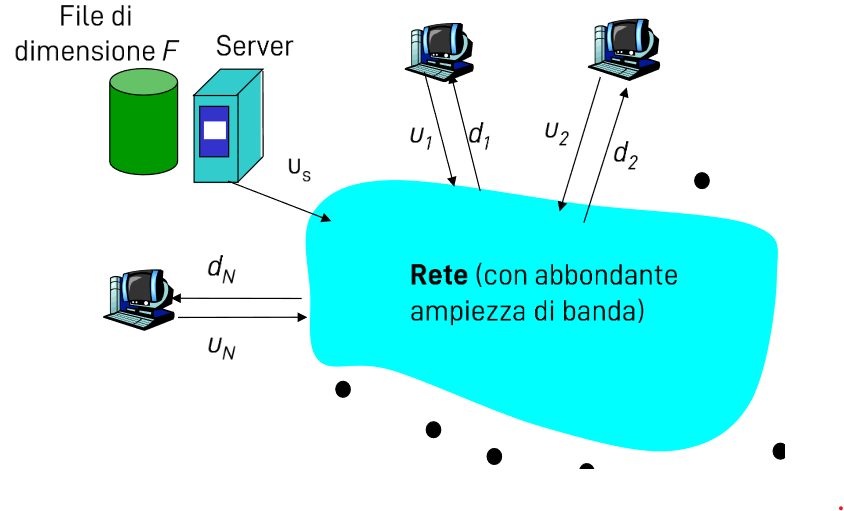
\includegraphics[width=0.5\textwidth]{02/reteP2P.png}
            \caption{Distribuzione di file in modalità \texttt{P2P}}
        \end{figure}
        \paragraph{Domanda:} Tenendo a mente la soprastante figura, ci si può chiedere: Quanto tempo ci vuole per distribuire un file da un server a $ N $ \textit{peer}?\newline
        Consideriamo: \textbf{$U_s$} il \textit{bitrate} in uscita del collegamento di accesso del server, \textbf{$U_i$} bit rate di upload del collegamento di accesso dell \textit{i}-esimo \textit{peer} e \textit{$d_i$} il \textit{bitrate} di download del collegamento di accesso dell \textit{i}-esimo \textit{peer}.
        \paragraph{Soluzione \textit{server-client}} In una architettura \textit{server-client} il tempo di distribuzione è dato dal server che deve inviare $N$ copie moltiplicato per la dimensione del file $F$ il tutto diviso per il \textit{bitrate} in uscita del server $U_s$, quindi in formula: $T=\frac{N\cdot F}{U_s}$. Ora il client $i$-esimo impiega il tempo $F/d_i$ per scaricare il file. Per calcolare il tempo per distribuire il file $F$ su $N$ client è uguale al massimo tra il tempo impiegato dal server per la trasmissione ($U_s$) e dal tempo massimo impiegato da un client per scaricare il file ($d_i$), quindi $d_{cs} = \max\left\{\frac{F}{U_s}, \frac{F}{\min(d_i)}\right\}$. Notare come il tempo di distribuzione aumenta linearmente rispetto al numero di \textit{peer}.
        \paragraph{Soluzione per \textit{P2P}} In una architettura \textit{P2P} per calcolare il tempo di distribuzione dobbiamo prima sapere quanto tempo impiega \textit{server} per inviare la prima copia del file $ T_s = \frac{F}{U_s} $ e poi necessitiamo di sapere quanto tempo impiega l'\textit{i}-esimo client per scaricare il file: $T_i= \frac{F}{d_i} $. Dato che poi il \textit{peer} che ha scaricato il file poi può trasmetterlo a sua volta allora il puù veloce tasso di \textit{upload} è: $U_s+\sum_iU_i $. Il tempo totale è dato dunque dal massimo tra: tempo di invio prima copia, tempo massimo di un peer e il tempo di invio di tutte le copie ($\frac{NF}{U_s\sum_iU_i} $), quindi in modo formulare: $ d_{P2P}=\max\left\{\frac{F}{U_s}, \frac{F}{\min(d_i)}, \frac{NF}{U_S+\sum_iu_i}\right\} $. Notare come il tempo di distribuzione a meno di un tempo costate per l'invio della prima copia si riduce all'aumentare del numero di \textit{peer}.
        \subsubsection{BitTorrnet}
            \paragraph{Introduzione} Nel protocollo di \textit{BitTorrent} si usa la distribuzione di file in modo \texttt{P2P} ma sono presenti dei \textit{server} detti \textit{tracker} che mantengono una lista di \textit{peer} partecipanti alla rete. Un nuovo \textit{peer} che vuole scaricare un file si connette al \textit{tracker} e ottiene la lista che stanno scaricando il file. Il \textit{peer} scarica il file da più \textit{peer} contemporaneamente, andando quindi a costituire una rete \textit{torrent}.
            \paragraph{Caratteristiche} I file vengono divisi in \textit{chunk} da $ 256kB $, quando un peer entra a far parte del torrent non possiede nessun \textit{chunk}, dunque si registra al server \textit{tracker} che gli assegna una lista di \textit{neighbors} ovvero vicini dai quali scaricherà i \textit{chunk} del file, quando un \textit{chunk} è scaricato il \textit{peer} lo condivide con gli altri alimentando l'effetto \textit{tit-for-tat}. Una volta che il file è scaricato nella sua completezza il \textit{peer} può lasciare la rete egoisticamente (\textit{leech}) o contribuire a questa (\textit{seeder})
    \subsection{Ricerca delle informazioni}
        I sistemi di tipo \texttt{P2P} devono in qualche modo fornire un indice della posizione dei \textit{peer} e di in quali di questi si può trovare un particolare file, solitamente questo viene fatto attraverso una \textit{Distributed hash table}.
            \subsubsection{File sharing \textit{e-mule}}
                In un sistema come \textit{e-mule} l'indice tiene traccia dinamicamente della posizione dei file che i \textit{peer} condividono, questi condividono i file disponibili. Un nuovo \textit{peer} cerca nell'indice quello che vuole trovare e poi stabilisce una connessione diretta al \textit{peer} contenete il file cercato.
            \subsubsection{Messaggistica istantanea}
                Nel caso della messaggistica istantanea l'indice crea una corrispondenza tra utenti e posizione (ip), quando un utente si registra all'applicazione informa il server della sua posizione, per inviare un messaggio ad un utente il \textit{peer} chiede al server la posizione dell'utente e poi stabilisce una connessione diretta.
            \subsubsection{Directory centralizzata}
                Nel caso di \textit{napster} invece quando un \textit{peer} si connette alla rete informa il server centrale del suo indirizzo ip e del contenuto condiviso, se un altro \textit{peer} cerca il contenuto dal server centrale allora questo restituisce l'indirizzo ip del \textit{peer} che condivide il file e il \textit{peer} può scaricare il file direttamente.
                \paragraph{Problemi} In primo luogo questa \textit{directory centralizzata} costituisce un \textit{Single point of failure}, inoltre essendo un solo punto questo è un importante \textit{bottleneck} infine se vengono condivisi file protetti da \textit{copyright} il server centrale ne è responsabile.
            \subsubsection{\textit{Query flooding}}
                Un sistema che adotta il \textit{query flooding} è completamente distribuito senza un server centrale, ogni \textit{peer} mantiene un indice locale dei file condivisi e quando un \textit{peer} cerca un file invia una \textit{query} a tutti i \textit{peer} vicini che se non hanno il file cercato inoltrano la \textit{query} ai loro vicini e così via. Questo sistema è molto efficiente ma può generare un grande traffico di rete. Una volta trovato il file viene istituita una connessione diretta \texttt{TCP} tra i due \textit{peer}. Questo sistema è molto efficiente ma può generare un grande traffico di rete ed è soggetto ad attacchi di tipo \textit{DoS}, se viene richiesto un file inesistente la \textit{query} viene inoltrata a tutti i \textit{peer} della rete.
\section{Cloud Computing}
    \paragraph{Introduzione} Il \textit{cloud computing} prevede che uno o più \textit{server} reali, organizzati in una architettura ad alta affidabilità e fisicamente collocati in un \textit{data center} del fornitore del servizio. Il fornitore espone delle interfacce per elencare e gestire i propri servizi, un utente amministratore usa queste selezionando i servizi richiesti per accedervi o amministrarlo, infine un utente finale può accedere ai servizi tramite un'interfaccia web o un'applicazione.
    \paragraph{Criticità}
        \begin{itemize}
            \item \textbf{Privacy \& Sicurezza} - I dati sono memorizzati in un server remoto
            \item \textbf{Continuità del servizio} - I servizi sono soggetti a interruzioni e necessitano di connessione internet
            \item \textbf{Problemi internazionali di natura economico-politica} - I dati possono essere soggetti a leggi di paesi diversi
            \item \textbf{Difficoltà di migrazione} - I dati possono essere difficili da migrare una volta che sono stati caricati
        \end{itemize}
    \subsection{\textit{Content Delivery Network} - \texttt{CDN}}
        \paragraph{Introduzione} Una \textit{CDN} è un sistema di server distribuiti che lavorano insieme per fornire contenuti web ad utenti finali con prestazioni elevate e alta affidabilità. Una \textit{CDN} è composta da \textit{server} detti \textit{edge server} che sono distribuiti in tutto il mondo, un \textit{server} centrale detto \textit{origin server} che contiene i contenuti originali e un \textit{server} detto \textit{DNS server}
        \paragraph{Esempio} 
            \begin{itemize}
                \item Un utente richiede un oggetto
                \item Il \textit{DNS server} determina il \textit{edge server CDN} più vicino all'utente
                \item Il \textit{edge server} richiede l'oggetto all'\textit{origin server} e lo memorizza
                \item Il \textit{edge server} invia l'oggetto all'utente
                \item Il \textit{edge server} memorizza l'oggetto per un certo periodo di tempo
                \item Se un altro utente richiede lo stesso oggetto il \textit{edge server} lo invia direttamente
                \item Se l'oggetto non è più richiesto il \textit{edge server} lo elimina
                \item Se l'oggetto cambia il \textit{edge server} lo richiede all'\textit{origin server}
            \end{itemize}
    
    \paragraph{Conclusione} "There is no cloud, it's just someone else's computer"
\end{document}